%---------------------------------------------------------------------
%
%                          Capítulo 3
%
%---------------------------------------------------------------------


\chapter{A \textit{Candida albicans} PeptideAtlas}
%\cabeceraEspecial{A \textit{Candida albicans} PeptideAtlas}

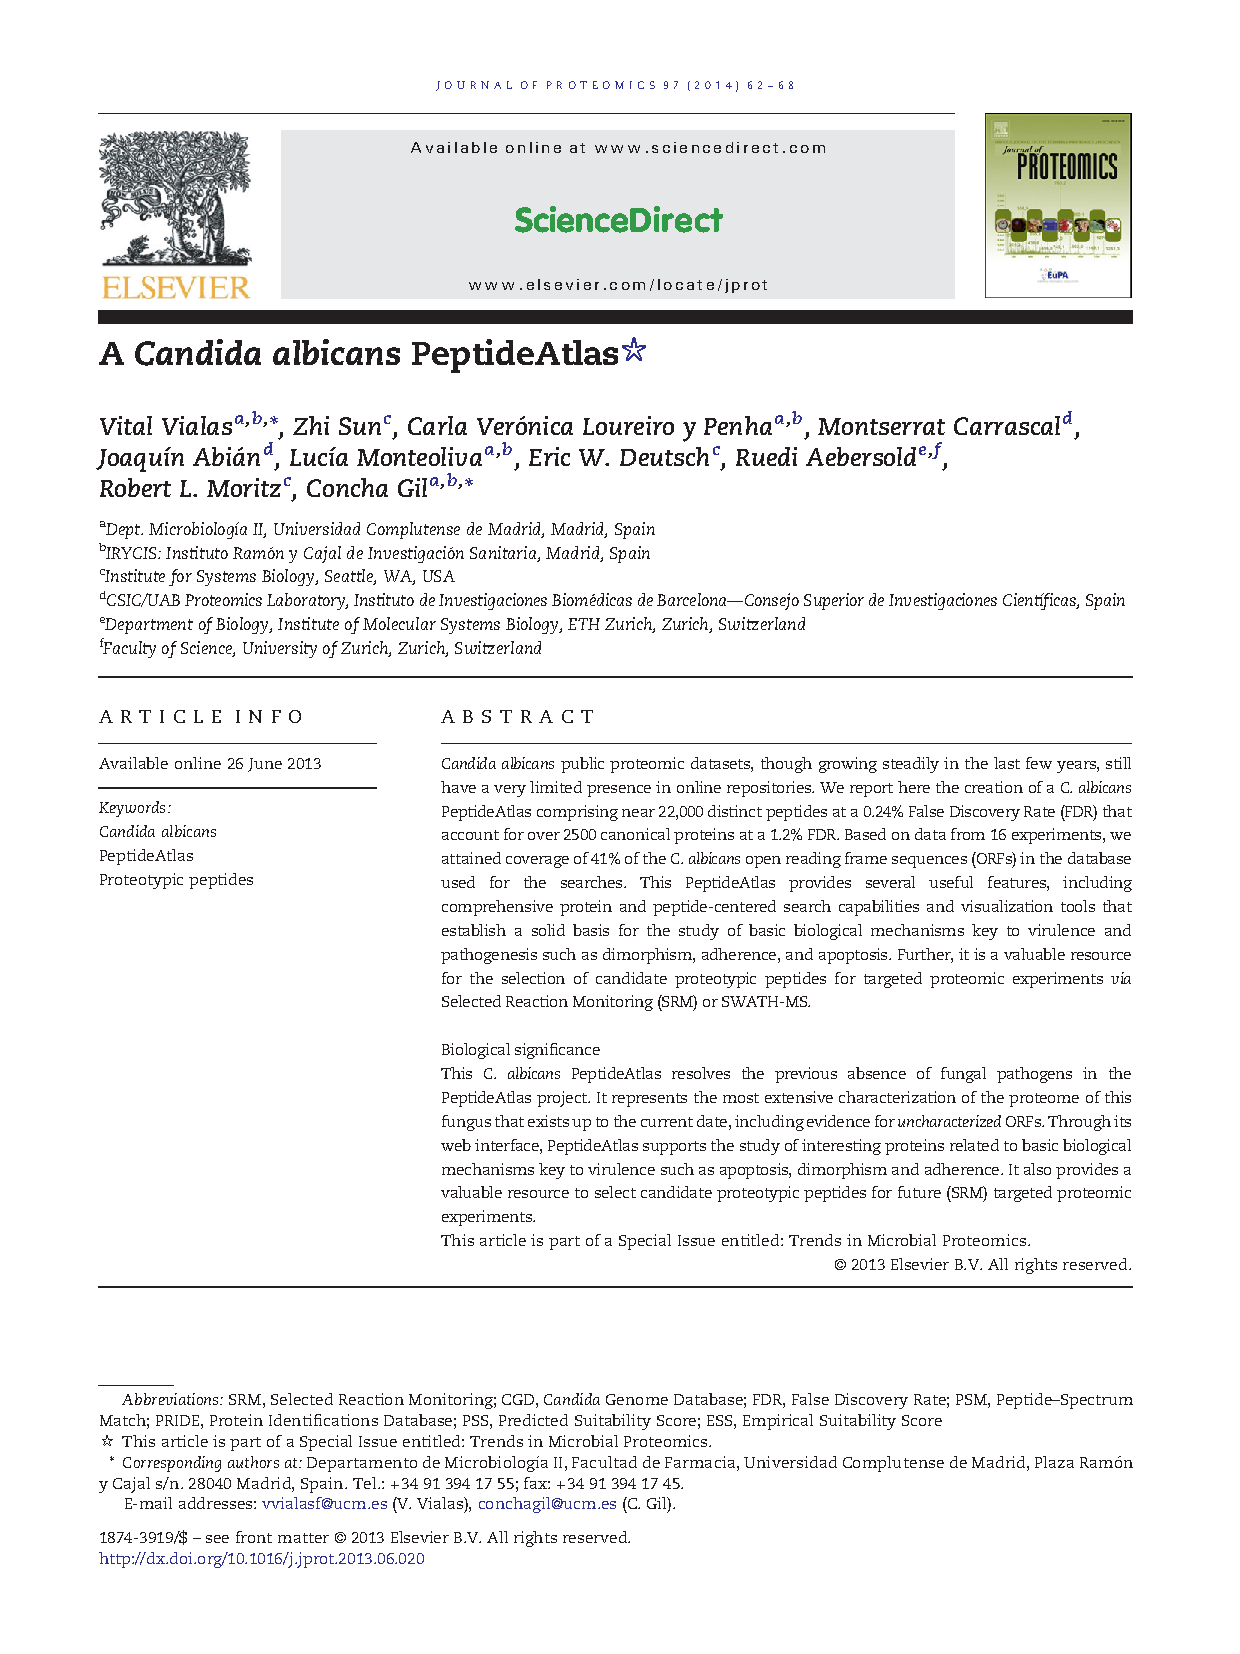
\includepdf[pages=-,scale=.8,pagecommand={}]{Capitulos/Vialas_2013_PeptideAtlas_JProteomics.pdf}


%\begin{FraseCelebre}
%\begin{Frase}
%...
%\end{Frase}
%\begin{Fuente}
%...
%\end{Fuente}
%\end{FraseCelebre}

%\begin{resumen}
%...
%\end{resumen}


%-------------------------------------------------------------------
\section{}


%-------------------------------------------------------------------
\label{cap2:sec:}

...

%-------------------------------------------------------------------
%\section*{\NotasBibliograficas}
%-------------------------------------------------------------------
%\TocNotasBibliograficas

%Citamos algo para que aparezca en la bibliografía\ldots
%\citep{ldesc2e}

%\medskip

%Y también ponemos el acrónimo \ac{CVS} para que no cruja.

%Ten en cuenta que si no quieres acrónimos (o no quieres que te falle la compilación en ``release'' mientras no tengas ninguno) basta con que no definas la constante \verb+\acronimosEnRelease+ (en \texttt{config.tex}).


%-------------------------------------------------------------------
%\section*{\ProximoCapitulo}
%-------------------------------------------------------------------
%\TocProximoCapitulo

...

% Variable local para emacs, para  que encuentre el fichero maestro de
% compilación y funcionen mejor algunas teclas rápidas de AucTeX
%%%
%%% Local Variables:
%%% mode: latex
%%% TeX-master: "../Tesis.tex"
%%% End:
